\iffalse
\let\negmedspace\undefined
\let\negthickspace\undefined
\documentclass[journal,12pt,twocolumn]{IEEEtran}
\usepackage{cite}
\usepackage{amsmath,amssymb,amsfonts,amsthm}
\usepackage{algorithmic}
\usepackage{graphicx}
\usepackage{textcomp}
\usepackage{xcolor}
\usepackage{txfonts}
\usepackage{listings}
\usepackage{enumitem}
\usepackage{mathtools}
\usepackage{gensymb}
\usepackage{comment}
\usepackage[breaklinks=true]{hyperref}
\usepackage{tkz-euclide}
\usepackage{listings}
\usepackage{gvv}
\def\inputGnumericTable{}
\usepackage[latin1]{inputenc}
\usepackage{color}
\usepackage{array}
\usepackage{longtable}
\usepackage{calc}
\usepackage{multirow}
\usepackage{hhline}
\usepackage{ifthen}
\usepackage{lscape}

\newtheorem{theorem}{Theorem}[section]
\newtheorem{problem}{Problem}
\newtheorem{proposition}{Proposition}[section]
\newtheorem{lemma}{Lemma}[section]
\newtheorem{corollary}[theorem]{Corollary}
\newtheorem{example}{Example}[section]
\newtheorem{definition}[problem]{Definition}
\newcommand{\BEQA}{\begin{eqnarray}}
\newcommand{\EEQA}{\end{eqnarray}}
\newcommand{\define}{\stackrel{\triangle}{=}}
\theoremstyle{remark}
\newtheorem{rem}{Remark}

%\bibliographystyle{ieeetr}
\begin{document}
%

\bibliographystyle{IEEEtran}


\vspace{3cm}

\title{
%	\logo{
Assignment-2

\large{EE:1205 Signals and systems}

Indian Institute of Technology, Hyderabad
%	}
}
\author{Sai Preetam Umesh Sasankota

EE23BTECH11221
}	



% make the title area
\maketitle

\newpage

%\tableofcontents

\bigskip

\renewcommand{\thefigure}{\theenumi}
\renewcommand{\thetable}{\theenumi}
	
\section{Question 1.2.4}
How many terms of the AP : 9, 17, 25, . . . must be taken to give a sum of 636?
\section{Solution}
\fi

\begin{table}[ht]
  \centering
  \begin{tabular}{|c|c|c|}
    \hline
    Parameter & Description & Value \\
    \hline
     x(0) & First Term & 9\\
     \hline
     d & Common Difference & 8\\
    \hline
    $S_n$ & Sum of n terms & 636\\
    \hline
  \end{tabular}
  \vspace{2mm}
  \caption{Parameter Table}
\end{table}
We know the formula
\begin{align}
S_n = \frac{\brak{n+1}}{2}[2x\brak{0}+d\brak{n}]
\end{align}
Putting in values from the table\\
\begin{align}
  636 = \frac{(n+1)}{2}\sbrak{18 + 8n} \\
  636 = \brak{n+1}\sbrak{4n + 9}\\
  4n^2 +13n -627= 0
\end{align}
On solving this quadratic equation, we get roots\\ $ n = -12.5$ and $ n = 11$\\
\\
Since we are looking for positive terms of n, we remove the negative root
\begin{align}
\implies n = 11
\end{align}
$\therefore$ the total number of terms are 12
\\
\\
The Z-Transform of the above question is
\begin{align}
X\brak{z}= &\frac9{1-z^{-1}} + \frac{8z^{-1}}{\brak{1-z^{-1}}^{2}}
\end{align}
\begin{figure}[ht]
    \centering
    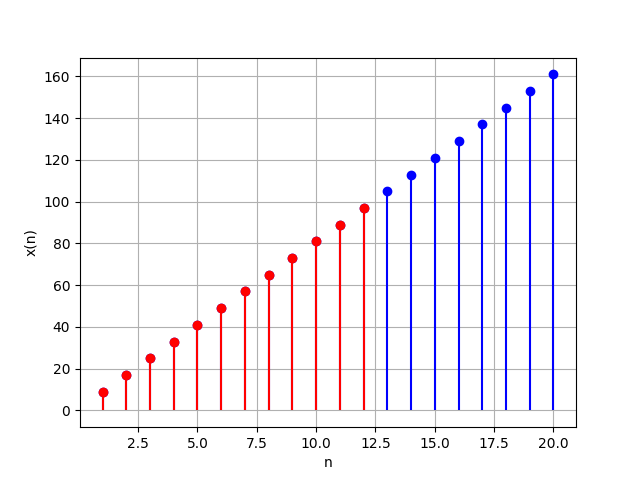
\includegraphics[width=\columnwidth]{ncert-maths/10/5/2/4/figs/fig1.png}
    \caption{Plot of x\brak{n} $vs$ n}
\end{figure}
%\end{document}
